\subsection{Ion Doppler and charge exchange recombination spectroscopy}\label{sec:ids}

Naturally occurring ion line emission in the plasma due to electron impact excitation and charge exchange with recycled neutral deuterium, is shifted in wavelength by ion velocity due to the Doppler effect and broadened due to the the thermal velocity distribution of the plasma ions. The broadening occurs since a portion of the observed line emission is red-shifted due to ions having velocity away from the observer and an portion is similarly blue-shifted. A net flow velocity in the plasma causes a net wavelength shift. Spectrally resolved measurements of this line emission can be observed using a spectrometer to determine the emitting ion population's density, velocity, and temperature.

\subsubsection{Physics principles of IDS}
The emission lines used to make theses observations can come from one of three reactions: electron impact excitation, charge exchange recombination, or radiative recombination. For the range of plasma temperature and density achieved in MST, %and in fusion physics in general, (This is not true for a detached diverter for example)
the radiative recombination is a negligible contribution. Typical line emission from MST consist primarily of the result of electron impact excitation and neutral deuterium charge exchange reactions with impurities. The impurities themselves are either atmospheric contaminants (like oxygen) or sourced from limiter sublimation (carbon) and wall sputtering (aluminum). Since this line emission is naturally occurring in the plasma, only a spectrometer and appropriate viewing optics are necessary to observe the emission to obtain information about the plasma. But ion Doppler spectroscopy using naturally-emitted line emission integrates light emitted from the entire plasma volume along the line of sight which is typically not uniform. This means the measurements are not localized except by the emission shells that form for partially-ionized ions in the temperature gradient regions of the plasma. Interpreting this emission requires detailed calculations of ion charge state which depends on the electron temperature and density as well as the neutral deuterium density and it can be a challenge to interpret measurements made. 

Charge exchange recombination spectroscopy (CHERS, or CER) is a special case of Doppler spectroscopy where a neutral beam is used to stimulate charge exchange emission along its path, allowing the spectrometer to make localized measurements where the beam and line of sight intersects. The Doppler shift due to the line-of-sight velocity of an emitting ion is 
\begin{align}
    \Delta\lambda = \lambda_0 \frac{v}{c}.
\end{align}
If we assume a Maxwellian distribution of emitting ions, then the lineshape of the spectral radiance is 
%altered from the $R(\lambda) = I_0\delta(\lambda_0)$ to 
% Technically, there is always some broadening, no matter how small. Even for very cold ions in atomic traps there is broadening due to quantum mechanical uncertainty effects referred to as "natural broadening."
%--
%Got it. -Xing
\begin{align}
    R(\lambda | v, T, I_0) &= \frac{I_0}{\sigma_\text{th} \sqrt{2\pi}}I_0 e^{\frac{-(\lambda-\lambda_c)}{2\sigma_\text{th}^2}}\\
    &\text{where:}\\
    I_0 &= n_{\text{imp}}n_s \left< \sigma v \right>^* &\text{is the total intensity}\\
    \sigma_\text{th} &= \frac{\lambda_0}{c}\sqrt{\frac{kT_\text{imp}}{m_{\text{imp}}}} &\text{is the thermal broadening, and}\\
    \lambda_c &= \lambda_0(1+\frac{\left< v_\text{imp} \right>}{c}) &\text{is the velocity shifted wavelength.}
\end{align}
Additionally, $n_s$ is the density and $\left<\sigma v\right>$ is the effective reaction rate (with branching fraction modification) of the emission generating reaction, $T_\text{imp}$, $<v_\text{imp}$, and $m_\text{imp}$ are the impurity temperature, velocity, and mass. This equation only considers thermal broadening of the line emission. One advantage that can be seen from this formula is the fact that the 3 plasma parameters of interest can be separated easily for analysis. For example, this thesis uses Doppler spectroscopy to look at impurity temperature, thus absolute calibration of wavelength is unimportant for this work as it effective folds into the $\lambda_c$ parameter. In general, the temperature corresponds to width, velocity to total shift, and density to the integrated radiance. 

Modelling charge exchange requires a bit of special consideration regarding both the isolation of the charge exchange emission, as well as the effect of fine structure broadening. To start, the charge exchange emission observed is contaminated by the same emission line excited through electron impact, referred to as background emission. To extract the local plasma information from the charge exchange emissions, the spectrometer also needs a 'reference' sight-line that looks at (effectively) the same plasma but in the absence of the beam. On MST this is done by having a second parallel sight-line offset about 2~cm toroidally. This way, the background emission can be fitted to a spectrum model and then incorporated into the combined charge exchange and background model for the measurements' sight-line. The second consideration has to do with fine structure of the emission line itself. Ultimately, line emission is the result of a bound electron dropping from one energy state to another and emitting a photon of energy equal to the difference of the energy levels. The energy states associated with primary quantum number $n$ consist of sub-levels due to the interaction of the electron orbital angular momentum with the spin angular momentum. The quantization of the angular momentum introduces the other quantum numbers, $l$, and $s$. Each of the energy sub-levels is also Doppler broadened effectively turning the line emission spectrum into the sum of many Gaussians, known as fine structure. The sub-levels associated with the spin number $s$, is due to Zeeman splitting, and the energy effect is small due to the relatively low magnetic field, and is not significant for the broadening calculations. The angular quantum number $l$ and the energy sub-levels associated have a significant effect on emissions, and charge exchange emissions especially.  Then, it is important to know the relative wave lengths and amplitudes of these component Gaussian emissions. But these can be difficult to calculate analytically as the probability of populating a certain fine structure level is complex and has many dependencies. These calculations have been performed elsewhere\cite{Isler1994}, this thesis instead relies on the Atomic Data and Analysis Structure (ADAS) database for the relative population of the fine structure states\cite{Summers2004}. 

\begin{figure}[!htb]
	\centering
    \begin{subfigure}[t]{0.5\textwidth}
        \centering
        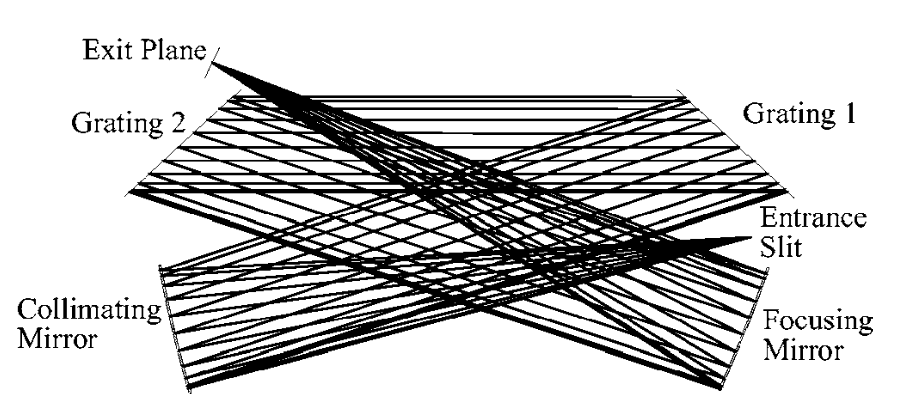
\includegraphics[width = \textwidth]{implementation/diagnostics/idsii_trace.png}
        \caption{Optical layout of IDS-II via ZEMAX}
    \end{subfigure}%
    ~ 
    \begin{subfigure}[t]{0.5\textwidth}
        \centering
        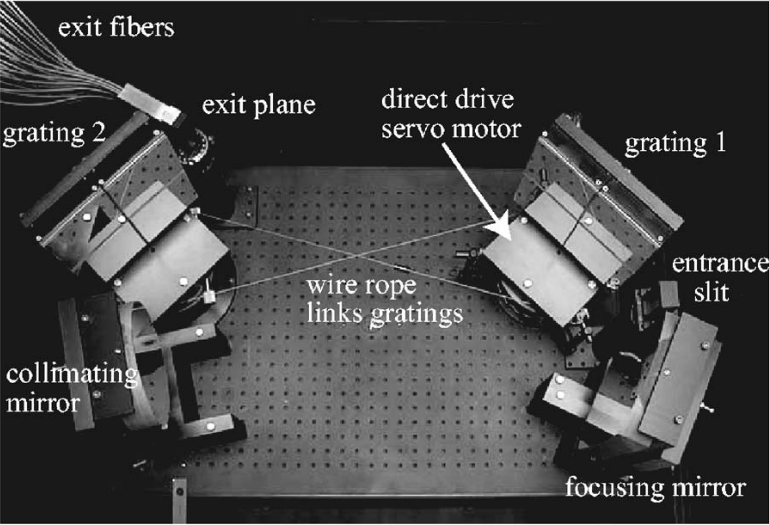
\includegraphics[width = \textwidth]{implementation/diagnostics/idsii_photo.png}
        \caption{Photograph of IDS-II layout}
    \end{subfigure}
	\caption[IDS-II optical layout]{IDS-II optical layout. Reproduced from Craig et al. \cite{Craig}}
	\label{fig:IDS-II}
\end{figure}

\subsubsection{Doppler spectroscopy hardware on MST}
On MST, ion Doppler spectroscopy is performed using the IDS-II (ion Doppler spectrometer, mkII). It is a custom built, high throughput spectrometer optimized for the 343~nm C~VI line, but it could be used for any viable emission line between 200~nm and 480~nm. This spectrometer can simultaneously measure emission from light collected along two optical views, either for the measurement and the reference views used for Charge exchange recombination spectroscopy, or two passive Doppler spectroscopy locations simultaneously. It uses a double grating Czerney-Turner design to achieve a high resolving power ($\lambda/\Delta\lambda \sim 5600$) while each of the gratings are actually a mosaic of 4 gratings, giving an large total area in order to achieve the high {\'e}tendu of 0.40 mm$^2$sr per view(see figure \ref{fig:IDS-II}). It uses a series of photo-multiplier tubes (PMTs) to measure the spectral radiance, allowing the system to achieve an effective data rate of up to 100~kHz in high current plasmas\cite{Craig}. Recent improvements improvements to the frequency response of the transimpedance-amplifiers have allowed fluctuation measurements up to 400~kHz\cite{Nishizawa2016}.


\begin{table}[h!]
    \centering
    \begin{tabular}{||c|c|c||}
        Chord \# & r/a & $\rho_v/a$\\
        \hline 
        1 & -0.91 & -0.92 \\
        2 & -0.76 & -0.80 \\
        3 & -0.58 & -0.64 \\
        4 & -0.41 & -0.48 \\
        5 & -0.24 & -0.32 \\
        6 & -0.07 & -0.15 \\
        7 & 0.11 & 0.03 \\
        8 & 0.28 & 0.20 \\
        9 & 0.45 & 0.37 \\
        10 & 0.62 & 0.55 \\
        11 & 0.80 & 0.75
        
    \end{tabular}
    \caption[IDS-II view chord locations]{IDS-II poloidal viewing chord locations. The $\rho/a$ refers to average magnetic flux surface location in axisymetric plasmas.}
    \label{tab:ids_chord_loc}
\end{table}

The IDS-II system has 11 poloidal viewing chords available, listed in table \ref{tab:ids_chord_loc}. It also has toroidal views available, but they are not used for this project since over the time scales studied the ion temperature is isotropic. 

A diagnostic neutral beam (DNB) is used to inject neutral particles to make localized CHERS measurements. The 'diagnostic' in it's name refer to the fact that the beam current is small such that it does not effectively perturb the plasma being observed, in comparison with heating and fueling beams that are designed to increase the temperature and density of the plasma. The DNB on MST is a nominally 50 ~keV, 4~A hydrogen neutral beam with a pulse length of 20~ms\cite{Feng2016}. The beam energy is optimized for the C$^{6+}$ charge exchange emissions which has a peak reaction rate at 45-50~keV. The beam has recently undergone a refit and the beam composition is measured to be about 75\% at full energy, 20\% at half energy and 5\% at a third energy.\cite{Feng2016}

\subsubsection{Line fitting and ensemble analysis}

This work uses the CHERS data obtained in two different modes and a brief discussion of the line fitting and ensembling techniques is needed to place them in context. The raw signals from the PMTs are digitized at 1MHz, but as discussed above, the spectrometer is designed for data-rates up to 100kHz; the difference is account for in the analysis algorithm. A linearized fluctuation analysis technique alternative to the one described here has been developed to analyze fluctuations up to 400kHz\cite{Nishizawa2017}, however this work focuses on the slower dynamics of the quai-equilibrium values and does not use this alternative. The default method starts by converting the 1MHz data into intensity through gain calibration values, then they are summed into time bins at the desired data frequency (1kHz to 100kHz are common), and subsequently, its photon-counting uncertainty is calculated from calibration (described in detail in T. Nishizawa's thesis\cite{Nishizawa2018}). Afterwards, a piece of code calculates the intensity that each PMT channel 'should' measure at a given temperature, velocity, and amplitude, but also accounting for fine structure and instrumental transfer function. A \chisq value is calculated from this model and the actual measurement, and a nonlinear optimization function is used to find the parameters at which the \chisq\ is minimized. If data analyzed is from two passive IDS views, they are fitted independently the same way. However, if a CHERS measurement is being analyzed, then the passive view (the reference) is analyzed as above, and the active view analysis incorporates this result. It does this by adding the passive contribution to the modeled intensity used to calculate the \chisq\ for the active view. Note that the fine structure for the passive emission and the active can be different as they are difference processes, but the instrumental transfer function are dependent on the view not the process. With this addition, the \chisq\ for the active channel is minimized and the analysis complete.

%%Hey Mark, this section below is going to change significantly, possibly disappear. 
Ensembling of data across multiple shots are used to improve the uncertainty of the measurements. The uncertainty for a particular fit is calculated using the co-variance of the \chisq as a function of the fitting parameters. In effect evaluating the 'width' of the \chisq well in each dimension. If the plasma conditions are perfectly repeatable within the ensembled shots, then the uncertainty of the ensemble can be calculated as the uncertainty of the mean, ie. $\sigma_{\text{ens}} = \frac{\Sigma \sigma}{\sqrt{N}}$. However, the shot to shot variation is not insignificant and the total uncertainty presented is $\sigma_{\text{ens}} = \sqrt{ (\frac{\Sigma \sigma}{\sqrt{N}})^2 + \sigma_{\text{shot to shot}}^2}$, and the shot to shot variation is characterized by the standard deviation of the average ion temperature during the PPCD period of each shot in the ensemble.

This method of uncertainty estimation is appropriate for the relatively slow 10kHz fits used for the model comparison work. However, the m = 0 burst analysis presented in chapter \ref{ch:m0} uses fast 50kHz fits, ensembled over m = 0 burst events. The shorter integration time used for the faster fitting means that each fits are noisy enough that sometimes the \chisq 'well' is poorly formed. Also, the burst to burst variation can be large and changes over the burst period. Hence, the uncertainty on the bursts are presented using the upper and lower values that bounds a 67.8\% of the points in the ensemble (\textit{i.e.} 1 sigma). This is chosen instead of the standard deviation value during the burst itself, the distribution of temperature values of a particular ensembled 'bin' tends to be skewed. 